\documentclass[11pt,a4j]{jsarticle}

\usepackage{float,array,booktabs,here}
\usepackage{amsmath}
\usepackage[dvipdfmx]{graphicx}
\usepackage[top=15truemm,bottom=20truemm,left=15truemm,right=15truemm]{geometry}
\usepackage{url}
\usepackage{listings}


\makeatletter
\newcommand{\figcaption}[1]{\def\@captype{figure}\caption{#1}}
\newcommand{\tblcaption}[1]{\def\@captype{table}\caption{#1}}
\makeatother

\newcommand{\Maru}[1]{\ooalign{
\ifnum#1<10 \hfil\resizebox{.9\width}{.85\height}{#1}\hfil
\else
\hfil\resizebox{.6\width}{.8\height}{#1}\hfil
\fi
\crcr
\raise.1ex\hbox{$\bigcirc$}}}


\begin{document}

% \title{フィルター}
% \author{hogehoge}
% \date{2015年5月9日}
% \maketitle


\section{目的}

光センサの一つであるフォトリフレクタを用いて実験を行って、IoTへの理解を深める。

\section{理論}
\label{sec:理論}

\subsection{フォトリフレクタ}
\label{sub:フォトリフレクタ}
フォトリフレクタは赤色LEDとフォトトランジスタからなるセンサーである。
赤色LEDから照射された赤外光の反射の変化で物体までの距離を計測することが可能である。
フォトリフレクタは安く、またサイズも小さいことから広く利用されている。


\section{実験方法}
\label{sec:実験方法}

\subsection{フォトリフレクタを用いた回路の作成}
\label{sub:フォトリフレクタを用いた回路の作成}

フォトリフレクタ、抵抗、可変抵抗そしてジャンパ品で構成される回路を
指定されたように回路を組んで半田付けを行った。

\subsection{フォトリフレクタのキャリブレーション}
\label{sub:フォトリフレクタのキャリブレーション}

金属板を用意し、その間の距離を徐々に大きくし、距離と計測された電圧値を記録した。
この値を Scilab を用いてフィッティングを行った。

\section{結果}
\label{sec:結果}

\subsection{キャリブレーション}
\label{sub:キャリブレーション}

\begin{table}[H]
  \caption{計測された電圧と距離の関係}
  \label{tab:caribration}
  \small
  \begin{center}
      \begin{tabular}{cc|cc}
        \hline
        \toprule
        距離$\mathrm{d /mm}$ & 電圧値 $\mathrm{V / mV}$ & 距離$\mathrm{d /mm}$ & 電圧値 $\mathrm{V / mV}$ \\
        \midrule
        0	&	0	&	4	&	93	\\
        0.1	&	404	&	5	&	63	\\
        0.2	&	619	&	6	&	47	\\
        0.3	&	728	&	7	&	34	\\
        0.4	&	763	&	8	&	28	\\
        0.5	&	775	&	9	&	23	\\
        0.6	&	756	&	10	&	19	\\
        0.7	&	708	&	11	&	16	\\
        0.8	&	676	&	12	&	13	\\
        0.9	&	630	&	13	&	12	\\
        1	&	579	&	14	&	10	\\
        2	&	283	&	15	&	8	\\
        3	&	150	\\				 \hline
      \end{tabular}
  \end{center}
\end{table}



Scilabにて変数d,Vを作成し、表\ref{tab:caribration}のデータをそれぞれ入力した。
このデータに対し以下のコマンドを実行してグラフを作成した。グラフの結果を図\ref{fig:fig1}に示した。

\begin{lstlisting}[basicstyle=\ttfamily\footnotesize, frame=single, framesep=0pt]
  plot2d(d,V,style=[-9]);
\end{lstlisting}

\begin{figure}[H]
  \centering
  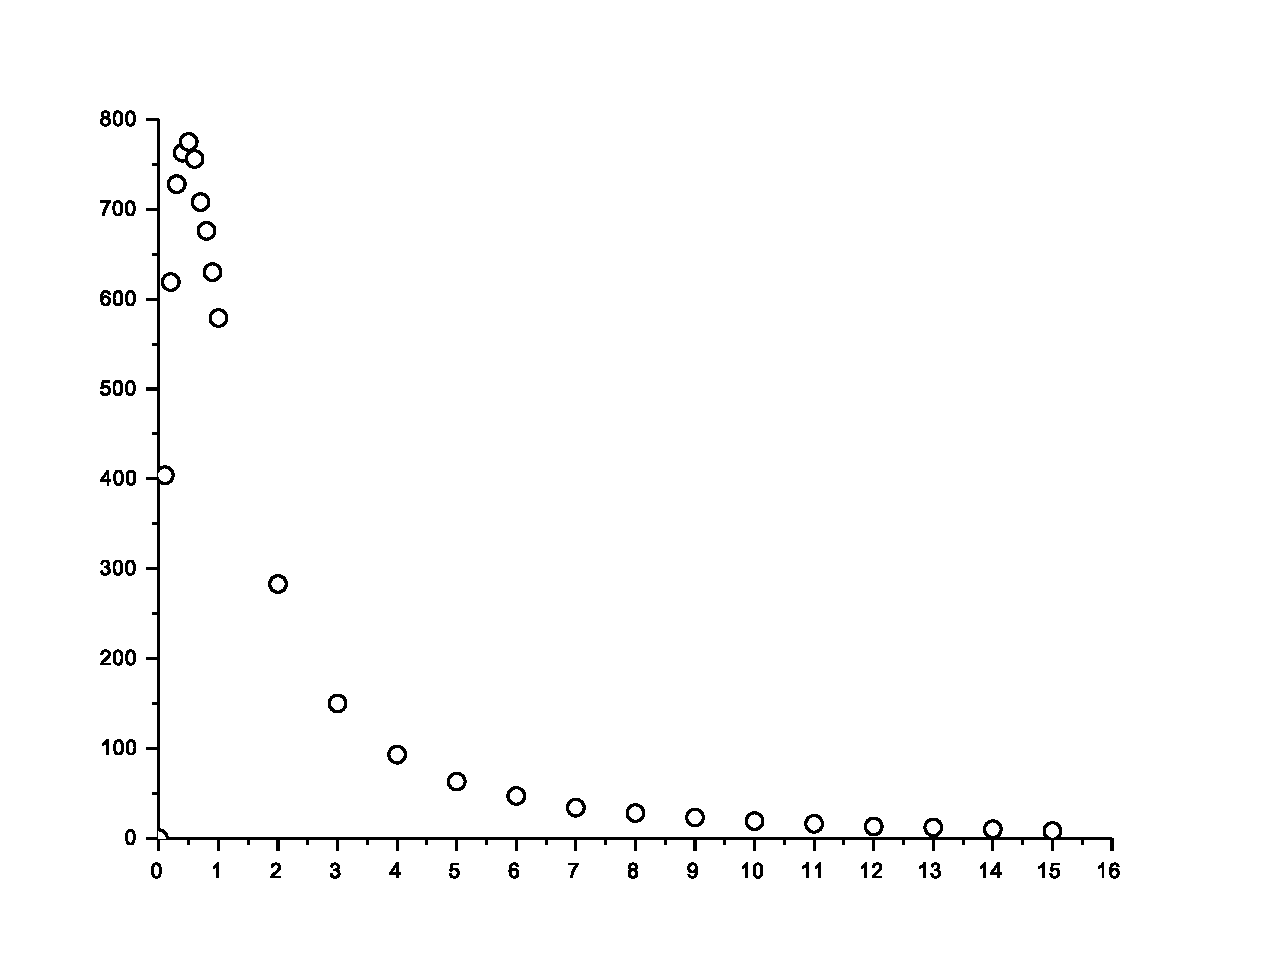
\includegraphics[height=70mm,bb=0 0 610 480]{image/fig1.pdf}
  \figcaption{電圧と距離の関係のグラフ}
  \label{fig:fig1}
\end{figure}

次に表\ref{tab:caribration}のデータを次のコマンドで変形し、
x, y, Xに代入した。

\begin{lstlisting}[basicstyle=\ttfamily\footnotesize, frame=single, framesep=0pt]
  x=d.^(2/3)./V.^(2/3);
  y=d.^2;
  X=x;
\end{lstlisting}

行列Xの2列目にすべて1を入れた。
y及び行列Xから定数$\mathrm{a_1}$と$\mathrm{a_2}$を (1,1), (1,2) とする行列$\mathrm{a}$を計算した。
この時の(x, y) とフィッティングにより求めた (x, yfitting) のグラフは図\ref{fig:fig2}のようになる.

\begin{lstlisting}[basicstyle=\ttfamily\footnotesize, frame=single, framesep=0pt]
  a=inv(X`*X)*X`*y;
  plot2d(x,y,style=[-9]);
  y_fitting=a1*x+a2;
  plot(x,y_fitting);
\end{lstlisting}


\begin{figure}[H]
  \centering
  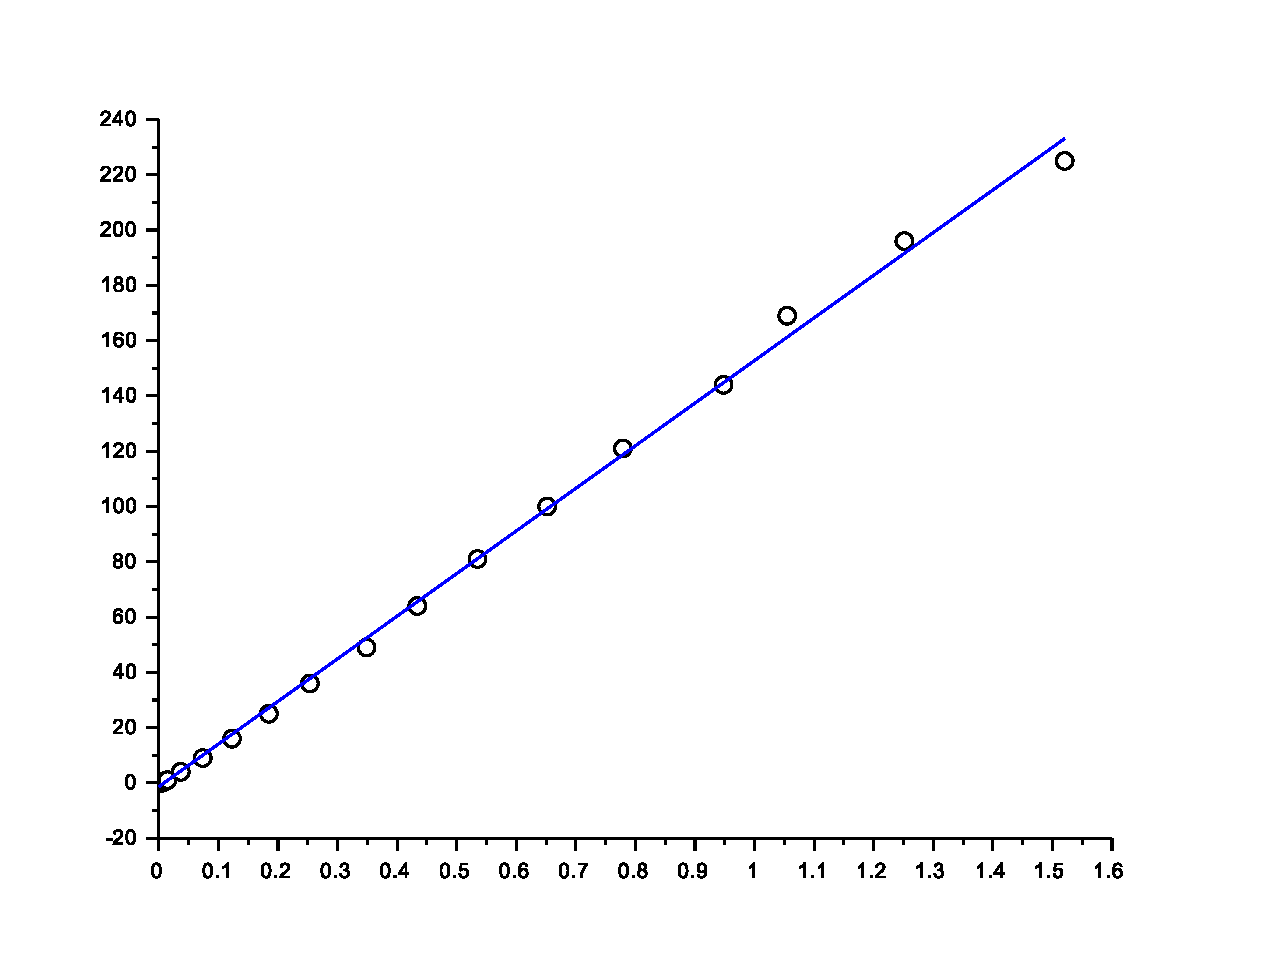
\includegraphics[height=70mm,bb=0 0 610 480]{image/fig2.pdf}
  \figcaption{(x,y)フィッティング}
  \label{fig:fig2}
\end{figure}

次に変数$\mathrm{a_1}$と$\mathrm{a_2}$にa行列の該当する値を代入する。

\begin{lstlisting}[basicstyle=\ttfamily\footnotesize, frame=single, framesep=0pt]
  a1=154.148883;
  a2=-1.33735;
\end{lstlisting}

よって求める式$\mathrm{V_{fitting}}$は以下のように求める。
元々のデータとフィッティングで得られた式をプロットしたものを、グラフを図\ref{fig:fig3}に示した。

\begin{lstlisting}[basicstyle=\ttfamily\footnotesize, frame=single, framesep=0pt]
  V_fitting=(k1*d)./(((d.^2)+k2).^(3/2));
  plot2d(d,V,style=[-9]);
  plot(d,V_fitting);
\end{lstlisting}

\begin{figure}[H]
  \centering
  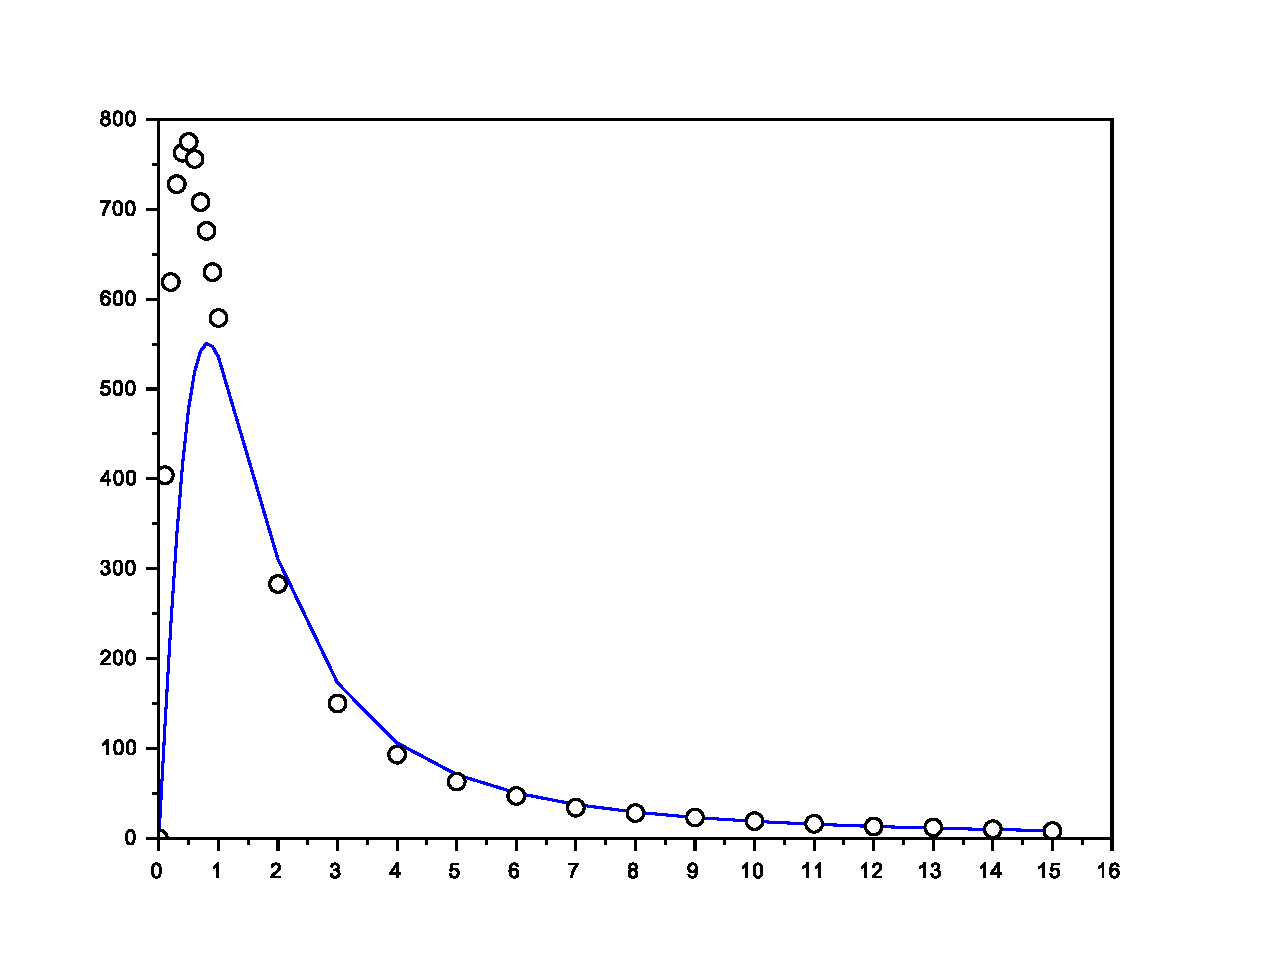
\includegraphics[height=70mm,bb=0 0 610 480]{image/fig3.pdf}
  \figcaption{電圧と距離の関係のグラフのフィッティング}
  \label{fig:fig3}
\end{figure}

\section{考察}
\label{sec:考察}

\subsection{フィッティグした式と実験地の誤差の要因}
\label{sub:フィッティグした式と実験地の誤差の要因}


フィッティグしたグラフと実測値では、電圧が最大となるとき、もっともフィッティングしたグラフの方が値が小さくなっている。
これは、dが小さい成分が原点付近に集中し、dが大きい成分が原点から離れた部分になっているので、
dが大きい値の重みが大きくなってしまっている。
そのため、dが小さい値ではフィッティングした式の誤差が大きくなってしまったのではないだろうかと考えられる。

\section{課題}
\label{sec:課題}

\subsection{フォトリフレクタで計測可能な実正解の素材}
\label{sub:フォトリフレクタで計測可能な実正解の素材}

計測可能な素材として、``陶芸品の乾燥の進行度''が考えられる。
陶芸は大まかに、粘土を整形、乾燥させる、焼くという工程が存在する。
この工程はすべて大事であるのだが、その中でも乾燥の進行度を正確に図ることができるというのは
とても大きな価値があるかと考えられる。
具体的な、進行度の測り方としては、粘土は完成するにつれてサイズが微妙に小さくなっていく。
そのため、微妙な変化に対して正確に値を測ることができるフォトリフレクタを用いることで可能となろう。

\subsection{フォトリフレクタを利用したアプリケーションの例}
\label{sub:フォトリフレクタを利用したアプリケーションの例}

アプリケーションの例として、エアコンなど、各種電化製品のスイッチのON/OFFの把握できるアプリケーション
を考えた。
電化製品は、本体に電源のON/OFFを知らせるためのランプがほとんど付いている。そのため、点灯部に貼り付けるような形で
フォトリフレクタを設置する。そして電源がONになっているタイミングとOFFになっている時の値を測り
それを記録させることでON/OFFを所得できるようになる。

このアプリケーションを、スマートフォンなど外部から監視できるようにすることで、つけ忘れなどを確認できるようになると思う

また、スマートフォン側のアプリケーションとして、自宅を離れる瞬間をチェックすることはWifiとの切断の
把握、GPSでの確認することが可能なので、離れるタイミングでフォトリフレクタの付いたAruduinoで
電源の確認を行い、付いていたら、スマートフォンアプリに通知をするなどとすることで、かなり可用性の高い
アプリケーションとなると思われる。


\begin{thebibliography}{9} %ケタ数(9:一桁、99:二桁)
\bibitem{sugiura} 杉浦裕太, ``実世界センシング'', 2016.
\end{thebibliography}

\end{document}
